\documentclass[]{book}
\usepackage{lmodern}
\usepackage{amssymb,amsmath}
\usepackage{ifxetex,ifluatex}
\usepackage{fixltx2e} % provides \textsubscript
\ifnum 0\ifxetex 1\fi\ifluatex 1\fi=0 % if pdftex
  \usepackage[T1]{fontenc}
  \usepackage[utf8]{inputenc}
\else % if luatex or xelatex
  \ifxetex
    \usepackage{mathspec}
  \else
    \usepackage{fontspec}
  \fi
  \defaultfontfeatures{Ligatures=TeX,Scale=MatchLowercase}
\fi
% use upquote if available, for straight quotes in verbatim environments
\IfFileExists{upquote.sty}{\usepackage{upquote}}{}
% use microtype if available
\IfFileExists{microtype.sty}{%
\usepackage{microtype}
\UseMicrotypeSet[protrusion]{basicmath} % disable protrusion for tt fonts
}{}
\usepackage[margin=1in]{geometry}
\usepackage{hyperref}
\hypersetup{unicode=true,
            pdftitle={Sleep quality analysis},
            pdfauthor={Arturo Laflor},
            pdfborder={0 0 0},
            breaklinks=true}
\urlstyle{same}  % don't use monospace font for urls
\usepackage{natbib}
\bibliographystyle{apalike}
\usepackage{longtable,booktabs}
\usepackage{graphicx,grffile}
\makeatletter
\def\maxwidth{\ifdim\Gin@nat@width>\linewidth\linewidth\else\Gin@nat@width\fi}
\def\maxheight{\ifdim\Gin@nat@height>\textheight\textheight\else\Gin@nat@height\fi}
\makeatother
% Scale images if necessary, so that they will not overflow the page
% margins by default, and it is still possible to overwrite the defaults
% using explicit options in \includegraphics[width, height, ...]{}
\setkeys{Gin}{width=\maxwidth,height=\maxheight,keepaspectratio}
\IfFileExists{parskip.sty}{%
\usepackage{parskip}
}{% else
\setlength{\parindent}{0pt}
\setlength{\parskip}{6pt plus 2pt minus 1pt}
}
\setlength{\emergencystretch}{3em}  % prevent overfull lines
\providecommand{\tightlist}{%
  \setlength{\itemsep}{0pt}\setlength{\parskip}{0pt}}
\setcounter{secnumdepth}{5}
% Redefines (sub)paragraphs to behave more like sections
\ifx\paragraph\undefined\else
\let\oldparagraph\paragraph
\renewcommand{\paragraph}[1]{\oldparagraph{#1}\mbox{}}
\fi
\ifx\subparagraph\undefined\else
\let\oldsubparagraph\subparagraph
\renewcommand{\subparagraph}[1]{\oldsubparagraph{#1}\mbox{}}
\fi

%%% Use protect on footnotes to avoid problems with footnotes in titles
\let\rmarkdownfootnote\footnote%
\def\footnote{\protect\rmarkdownfootnote}

%%% Change title format to be more compact
\usepackage{titling}

% Create subtitle command for use in maketitle
\newcommand{\subtitle}[1]{
  \posttitle{
    \begin{center}\large#1\end{center}
    }
}

\setlength{\droptitle}{-2em}
  \title{Sleep quality analysis}
  \pretitle{\vspace{\droptitle}\centering\huge}
  \posttitle{\par}
  \author{Arturo Laflor}
  \preauthor{\centering\large\emph}
  \postauthor{\par}
  \predate{\centering\large\emph}
  \postdate{\par}
  \date{2017-05-10}

\usepackage{booktabs}
\usepackage{amsthm}
\usepackage{multirow}
\usepackage{multicol}
\usepackage{float}
\usepackage{tabularx}
\makeatletter
\def\thm@space@setup{%
  \thm@preskip=8pt plus 2pt minus 4pt
  \thm@postskip=\thm@preskip
}
\makeatother

\begin{document}
\maketitle

{
\setcounter{tocdepth}{1}
\tableofcontents
}
\chapter{Description of the work}\label{description-of-the-work}

This work describes the progress that has been made so far in estimating
sleep quality, based on sleep hygiene factors. The characterization of
the phenomenon is being carried out in two stages, the first, described
in this work, has to do with the generation of a model that estimates
the quality of sleep and that has been trained with subjective data from
a questionnaire applied to 341 volunteers . The second stage is in
process, this stage includes a logbook that records the factors of a
person's sleep hygiene every day and the measurement of quality is not
subjective, but is measured by an electronic device. In this way, in the
end, an analysis of both characterizations will be made and a model will
be constructed that takes into account the two perspectives to obtain a
better approximation in their predictions.

\chapter{Introduction}\label{intro}

The monitoring of sleep and the estimation of sleep quality has become
relevant in recent years due to research that has positively correlated
poor sleep quality with various problems ranging from mild to serious.
Minor and short-term problems include lack of concentration, difficulty
remembering and learning new things and irritability, while more serious
problems talk about hypertension, type II diabetes, Alzheimer's and
other chronic degenerative diseases.

The intention of this work is to construct a model that infer the
quality of sleep of a person from the factors of the hygiene of the
sleep. The literature discusses at least 21 factors of sleep hygiene
that should be considered when studying the possible causes of a sleep
disorder, physicians conduct interviews and apply questionnaires to
their patients to investigate behaviors that favor or impair sleep
quality, and from there they begin to generate a clinical file that
allows them to diagnose or move to a second stage of the protocol that
consists of laboratory studies such as polysomnography or actigraphy.

This work is aimed at the prevention of poor sleep quality and the
possible prevention of a sleep disorder. It is a question of
constructing a model that estimates the quality of sleep from the most
relevant factors of sleep hygiene for a given population. The model will
acquire data of the hygiene of the dream by means of sensors coupled to
the surroundings of the user and will make an estimation of the quality
of the dream, later the user will give a qualification to his quality of
dream of such form that day to day the model is Adjustment to the
lifestyle and sleep patterns of the person and the person make changes
to that lifestyle, following model recommendations in such a way that
their quality of sleep is favored.

The first part in the construction of the model consisted of collecting
information through clinically proven questionnaires on the perception
of sleep quality and sleep hygiene in a sample of people as Section
\ref{data-adquisition} explains. With these data a study of the most
relevant factors was made so that of the 21 original sleep hygiene
factors that were taken from the literature, only the most relevant set
was selected (see Section \ref{feature-selection}). This will make it
possible to implement the model in a real system because a reduced
number of factors implies few sensors in the context of the user, which
translates into less design complexity, less intrusiveness and less
infrastructure cost.

After selecting the most relevant factors for the estimation of sleep
quality, we proceeded to test the model using the cross-validation
technique. This was done with two purposes. The first one was to
validate that the selection of factors was successful in verifying that
with the subset of variables the model predicts with more efficiency the
quality of sleep than when using the total factors. Second, this work
was useful to obtain the first performance analysis of three supervised
automated learning techniques to generate predictive models. The
techniques tested were artificial neural networks (ANNs), logistic
regression with regularization (LR) and vector supported machines (SVM).
The three techniques had an efficient behavior as can be seen in the
Section \ref{evaluation-of-efficiency} and are candidates for any of
them being chosen to be the basis of the model.

\hypertarget{data-adquisition}{\chapter{\texorpdfstring{\protect\hyperlink{data-adquisition}{Data
adquisition}}{Data adquisition}}\label{data-adquisition}}

\section{Questionnaire}\label{questionnaire}

In order to obtain data that contribute with evidence, regarding of
relations between Sleep Hygiene Factors (FSH) and the Quality of Sleep
(QS), we selected two questionnaires clinically used. The Sleep Hygiene
Index (SHI) and the Pitsburgh Sleep Quality Index (PSQI). As the
population where the new questionnaire would be applied is
Spanish-speaking and original questionnaires are in English language, we
proceed to do the process of translation. The valid process to obtain a
reliable translation consist of following stages: A person \texttt{A}
translate the questionnaires from English to Spanish, a person
\texttt{B} getback the spanish translation to the English language, and,
a person \texttt{C}, compare the questionnaire obtained by the
translation of the \texttt{B} person agains the original questionnaire.
The \texttt{C} person, writes comments regarding of those itemes that do
not match in meaning, corrections are done, and the process iterate
until reach a satisfactory result (see Fig. \ref{fig:double-tr}).

\begin{figure}

{\centering 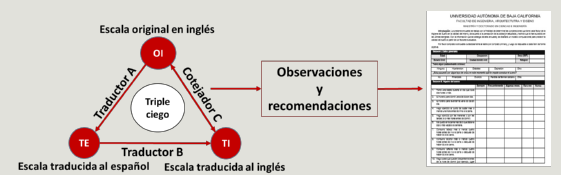
\includegraphics[width=0.8\linewidth]{images/double-translation} 

}

\caption{Double translation}\label{fig:double-tr}
\end{figure}

After this translation, the two questionnaires where joined in a single
questionnaire, adding a section in order to obtain demographic,
emoptional and health data of relevance to this study. The new
questionnaire was comformed by three sections. The first section has six
demographic items, one emotional and one health item, the second section
is the PSQI questionnaire that consists of 20 items, and, the third
section is the SHI whit a total of 21 items. In the end, the SHI survey
was left with 21 items, unlike the original that has 13, this has been,
only for data granularity reasons, however, the changes do not alter the
SHI objective. For example, item six of the original questionnaire that
asked about the use of tobacco, alcohol, or caffeine, became three items
to ask separately about the use of these three substances.

In the end, the questionnaire consisted of 47 items, divided into three
sections that are described later. The purpose of the questionnaire is
to collect data to be analyzed using automated learning techniques
(specifically the techniques of feature selection) to determine those
sleep hygiene factors that have a greater impact on the quality of sleep
from the respondent's perception. One of the specific objectives of this
research is to delimit the domain of input data to a subset of factors
that explain an appropriate percentage of the variance of the
phenomenon. The resulting factors will be used as the predictive
variables in the first stage of training of the inference model to
estimate the quality of sleep.

\subsection{Demographic emotional and health
data}\label{demographic-emotional-and-health-data}

\subsubsection{Demographic}\label{demographic}

In this section we ask about six relevant data that allow to understand
the context of respondent. The six variables are age, gender, ocupation,
kind of work, religion and civil status. Of this six variables,
\textbf{kind of work} provide relevant information to the study, since
the literature says that phisical activity improve the sleep quality
{[}cita{]} . The options for this question are: \emph{intellectual},
\emph{phisical}, \emph{more intellectual than phisical} and, \emph{more
phisical than intellectual}. The other variables in this section are for
exploration purposes regarding of sleep quality and sleep hygiene.

\subsubsection{Emotional}\label{emotional}

This variable asks to the respondent if he/she are in a crisis time. The
crisis can be financial, mourning, divorce, or other that can
significantly alter the quality of sleep. This answer is a target
population filter for this study. Data from people in this circumstances
are noisy to the study and should not be part of the data that will be
used for the analysis.

\subsubsection{Health}\label{health}

Similar than \emph{Emotional} variable, the health variable asks if the
respondent suffers from a chronic degenerative disease such as diabetes,
hypertension, depression or another that can directly or indirectly
alter the quality of sleep. Data from people suffering some disease are
removed before the analysis.

\subsection{Quality of Sleep}\label{quality-of-sleep}

The PSQI is considered the gold standard questionnaire to evaluate
subjective sleep quality \citep{Cameron2010}, and has been used to
estimate the quality of sleep in clinical and nonclinical population
\citep{mastin2006}, and has been referred by numerous researchs in
diverse sleep assessments \citep{bai2012}. This questionnaire evaluates
the quality of sleep using nineteen items grouped in seven components:
subjective sleep quality, sleep duration, sleep latency, sleep
disturbances, use of sleep medication, day time disfunction and sleep
latency. The questionnaire provide a baremo to score each component and
sumarize the final score resulting in a dicotomic varaible; \emph{-good
quality of sleep-} or \emph{-poor quality of sleep-} \citep{psqi1989}.
For the purposes of this study, eighteen of the nineteen items was used
in the second section, it fact does not affect the score results, since
that latter item is not taken into account for the computation of the
scale in the original questionnaire. On the other hand, the last item
has to do with specific sleep disorders, for example, \emph{-sleep
apnea-}, while this study seeks to understand sleep habits in healthy
people.

\subsection{Sleep Hygiene Index}\label{sleep-hygiene-index}

It is an instrument designed to measure the sleep hygiene behavior in a
nonclinical population. Its theoretical basis is in the criteria that
International Classification of Sleep Disorders (ICSD) uses to diagnose
an inadequate sleep hygiene. The scale has thirteen items and has
reported an internal validity of \(\alpha=0.71\), as well a high
reliability in test-retest evaluation\citep{mastin2006}.

For the purposes of this study and based on what the literature reports
regarding sleep hygiene factors, the following adjustments were made to
the instrument, without interfering with its essence:

\begin{itemize}
\item
  Following the structure and the meaning of the item four \emph{- I
  exercise to the point of sweating within 1 h of going to bed-}, two
  items were added: \emph{- I exercise to the point of sweating during
  the morning-} and \emph{-I exercise to the point of sweating during
  the afternoon.- }. The main purpose was to know whether the exercise
  in the morning or in the afternoon is directly correlated with sleep
  quality.{[}cita{]}
\item
  Item six of the original questionnaire that asked about the use of
  tobacco, alcohol, or caffeine, became three items to ask separately
  about the use of these three substances.
\item
  Item 11 in the original questionnaire asks about an uncomfortable
  bedroom, due to four environment factors. In the questionnaire for
  this study, four items was generated from this one.
\item
  Based on what the literature says about dinner type and schedule, and
  its negative impact on sleep quality, an item was added to the
  questionnaire
  \citep[Stefano2014,\citet{Irish2015},\citet{Wentz2011}]{Posner2011}.
\end{itemize}

\section{Validity and reliability}\label{validity-and-reliability}

After the instrument was completed, it was validated by five experts
that qualify each item on a escale of 1 to 5 for two metrics, clarity
and pertinence. All items were qualified as clear and relevant. with the
mean of 4.5 and 4.7 respectively. A sample of 30 people was randomly
selected to perform the pilot test and obtain the internal validity of
the instrument. Cronbach's alpha for the instrument after pilot test was
\(\alpha=0.68\). This \(\alpha\) value is acceptable and consistent with
that reported by \citep{mastin2006} for the SHI scale, with this we
proceeded to apply the questionnaire to a wider population to collect
the dataset with which the analyzes were made for the selection of
Variables that will be taken into account for the construction of the
model.

\section{Dataset}\label{dataset}

As a result of apply the questionnaire, a raw dataset \((m=342, n=47)\)
was obtained, this dataset, have missing data, some columns are no
significant in terms of variance, there exist data in a wrong format to
analyze, among other data quality issues. To obtain the dataset to the
feature selection analysis, it was neccesary a pre-process of data, what
included: The data quality analysis, the data quality plan to attend the
issues and the implementation of the data quality plan. After this
pre-process of data, the final dataset is conformed by one ID, 51
continuous and 10 categorical features grouped as shows the table
\ref{tab:dataset-columns-distribution}.

\begin{table}[ht]
\centering
\caption{Columns distribution by its nature}
\label{tab:dataset-columns-distribution}
\begin{tabular}{lrrr}
\hline
Group             & Categorical & Continuous & Total \\ \hline
ID                & 0           & 1          & 1     \\
Demographics data & 7           & 1          & 8     \\
PSQI              & 14          & 4          & 18    \\
SHI               & 21          & 0          & 21    \\
Scale PSQI        & 8           & 1          & 9     \\
Scale SHI         & 0           & 5          & 5     \\ \hline
Total             & 50          & 12         & 62    \\ \hline
\end{tabular}
\end{table}

The complete description of the dataset is in the tables
\ref{tab:demographic-feature-description},
\ref{tab:psqi-features-description},
\ref{tab:PSQI-Scale-features-description},
\ref{tab:SHI-feature-description} and
\ref{tab:SHI-scale-feature-description}. At the end, the dataset
contains 21 columns of main predictive variables (SHI), one column for
continuous target variable (SQTT), and, one column for categorical
target variable (SQCL). The other features in the dataset have diverse
purposes as the last column of each table describes.

\begin{table}[ht]
    \centering
    \caption{Demographic features description}
    \label{tab:demographic-feature-description}
    \begin{tabular}{|l|l|l|p{5cm}|p{4cm}|}
        \hline
        \multicolumn{1}{|c|}{\textbf{Grupo}} & \multicolumn{1}{c|}{\textbf{Feature}} & \multicolumn{1}{c|}{\textbf{Type}} & \multicolumn{1}{c|}{\textbf{Values}}                                                     & \multicolumn{1}{c|}{\textbf{Purpose}}                              \\ \hline
        ID                                   & EMAIL                                 & Text                               & inf                                                                                      & identificator                                                   \\ \hline
        \multirow{8}{*}{}         & DD1                                   & Continuous                         & {[}1-100{]}                                                                              & \multirow{6}{4cm}{Demographic data for statistical purposes only} \\ \cline{2-4}
        & DD2                                   &        & Female, Male                                                                             &                                                                 \\ \cline{2-2} \cline{4-4} 
        & DD3                                   &                                    & Student, Employer, Teacher, Independent professional, Other                              &                                                                 \\ \cline{2-2} \cline{4-4}
        & DD4                                   & \multirow{6}{*}{Categorical}                                  & Intellectual, Physical, More intellectual than physical, More physical than intellectual &                                                                 \\ \cline{2-2} \cline{4-4} {Demographic}
        & DD5                                   &                                    & SDA, Catholic, Jehovah's withess, Evangelic, Other                                       &                                       \\ \cline{2-2} \cline{4-4} 
        & DD6                                   &                                    & Married, Single, Divorced, Free Union, Other                                             &                                                                 \\ \cline{2-2} \cline{4-5} 
        & DD7                                   &                                    & No, Hypertension, Diabetes, Depression, Other                                            & Demographic information with filtering purposes                 \\ \cline{2-5} 
        & DD8                                   &                                    & No,Financial, Divorce process, Loss of Family, Other                                     & Financial,                                                      \\ \hline
    \end{tabular}
\end{table}

\begin{table}[ht]
    \centering
    \caption{PSQI features description}
    \label{tab:psqi-features-description}
    \begin{tabular}{|l|l|l|p{3cm}|p{5cm}|}
        \hline
        \multicolumn{1}{|c|}{\textbf{Group}} & \multicolumn{1}{c|}{\textbf{Feature}} & \multicolumn{1}{c|}{\textbf{Type}} & \multicolumn{1}{c|}{\textbf{Values}}                    & \multicolumn{1}{c|}{\textbf{Purpose}}                                                                              \\ \hline
        \multirow{18}{*}{PSQI}               & SQ1                                   & \multirow{4}{*}{Continuous}        & A real numer.   $ 0 \leq  SQ1 \leq 12 $                    & \multirow{18}{5cm}{Provide information to PSQI Scale. A 0 value is the best for sleep quality and 3 is the worst} \\ \cline{2-2} \cline{4-4}
        & SQ2                                   &                                    & An integer number. $ 0 \leq SQ2 \leq 60 $               &                                                                                                                 \\ \cline{2-2} \cline{4-4}
        & SQ3                                   &                                    & A real number. $ 0 \leq SQ3 \leq 12 $                      &                                                                                                                 \\ \cline{2-2} \cline{4-4}
        & SQ4                                   &                                    & A real number. $ 0 \leq SQ4 \leq 12 $                      &                                                                                                                 \\ \cline{2-4}
        & SQ5a                                  & \multirow{14}{*}{Categorical}      & \multirow{14}{3cm}{A level variable. $ 0 \leq SQ* \leq 3 $.} &                                                                                                                 \\ \cline{2-2}
        & SQ5b                                  &                                    &                                                         &                                                                                                                 \\ \cline{2-2}
        & SQ5c                                  &                                    &                                                         &                                                                                                                 \\ \cline{2-2}
        & SQ5d                                  &                                    &                                                         &                                                                                                                 \\ \cline{2-2}
        & SQ5e                                  &                                    &                                                         &                                                                                                                 \\ \cline{2-2}
        & SQ5f                                  &                                    &                                                         &                                                                                                                 \\ \cline{2-2}
        & SQ5g                                  &                                    &                                                         &                                                                                                                 \\ \cline{2-2}
        & SQ5h                                  &                                    &                                                         &                                                                                                                 \\ \cline{2-2}
        & SQ5i                                  &                                    &                                                         &                                                                                                                 \\ \cline{2-2}
        & SQ5j                                  &                                    &                                                         &                                                                                                                 \\ \cline{2-2}
        & SQ6                                   &                                    &                                                         &                                                                                                                 \\ \cline{2-2}
        & SQ7                                   &                                    &                                                         &                                                                                                                 \\ \cline{2-2}
        & SQ8                                   &                                    &                                                         &                                                                                                                 \\ \cline{2-2}
        & SQ9                                   &                                    &                                                         &                                                                                                                 \\ \hline
    \end{tabular}
\end{table}

\begin{table}[ht]
    \centering
    \caption{PSQI Scale features description}
    \label{tab:PSQI-Scale-features-description}
    \begin{tabular}{|l|l|l|p{3cm}|p{5cm}|}
        \hline
        \multicolumn{1}{|c|}{\textbf{Group}} & \multicolumn{1}{c|}{\textbf{Feature}} & \multicolumn{1}{c|}{\textbf{Type}} & \multicolumn{1}{c|}{\textbf{Value}}   & \multicolumn{1}{c|}{\textbf{Purpose}}    \\ \hline
        & SQDUR  &   &   & Results of SQ duration. A 0 value is the best for sleep quality and 3 is the worst.                                           \\ \cline{2-2} \cline{5-5} 
        & SQDIS    &      &    & Results of SQ disturbances. A 0 value is the best for sleep quality and 3 is the worst. \\ \cline{2-2} \cline{5-5} 
        \multirow{9}{*}{PSQI Scale} & SQLAT  & \multirow{7}{*}{Categorical}  &  \multirow{7}{3cm}{A level variable. $ 0 < SQ*\leq 3 $.}  & Results of SQ latency. A 0 value is the best for sleep quality and 3 is the worst.    \\ \cline{2-2} \cline{5-5} 
        & SQDD   &    &   & Results of SQ day dysfunction. A 0 value is the best for sleep quality and 3 is the worst. \\ \cline{2-2} \cline{5-5} 
 & SQSE                                  &                                    &                                                       & Results of SQ sleep efficiency. A 0 value is the best for sleep quality and 3 is the worst.                                   \\ \cline{2-2} \cline{5-5} 
        & SQSQ                                  &                                    &                                                       & Results of SQ sleep quality general perception of the respondent. A 0 value is the best for sleep quality and 3 is the worst. \\ \cline{2-2} \cline{5-5} 
        & SQMS                                  &                                    &                                                       & Results of SQ, needs meds. A 0 value is the best for sleep quality and 3 is the worst.                                        \\ \cline{2-5} 
        & SQTT                                  & Continuous                         & An integer value. $ 0 < SQTT\leq 21 $.                 & Total of PSQI                                                                                                                 \\ \cline{2-5} 
        & SQCL                                  & Categorical                        & A level value.                                        & Good/ Poor                                                                                                       \\ \hline
    \end{tabular}
\end{table}

\begin{table}[ht]
    \centering
    \caption{SHI features description}
    \label{tab:SHI-feature-description}
    \begin{tabular}{|l|l|l|l|l|}
        \hline
        \multicolumn{1}{|c|}{\textbf{Group}} & \multicolumn{1}{c|}{\textbf{Feature}} & \multicolumn{1}{c|}{\textbf{Type}} & \multicolumn{1}{c|}{\textbf{Values}} & \multicolumn{1}{c|}{\textbf{Purpose}}   \\ \hline
        \multirow{21}{*}{SHI}  & SHI  & \multirow{21}{*}{Categorical} & \multirow{21}{3cm}{A level variable. $ 0 < SH*\leq 4 $.} & \multirow{21}{5cm}{Predictive Features (Provide information for SHI scale). A 0 value is the best for sleep hygiene and 4 is the worst} \\ \cline{2-2}
        & SH2                                   &                                    &                                                        &                                                                                                                                         \\ \cline{2-2}
        & SH3                                   &                                    &                                                        &                                                                                                                                         \\ \cline{2-2}
        & SH4                                   &                                    &                                                        &                                                                                                                                         \\ \cline{2-2}
        & SH5                                   &                                    &                                                        &                                                                                                                                         \\ \cline{2-2}
        & SH6                                   &                                    &                                                        &                                                                                                                                         \\ \cline{2-2}
        & SH7                                   &                                    &                                                        &                                                                                                                                         \\ \cline{2-2}
        & SH8                                   &                                    &                                                        &                                                                                                                                         \\ \cline{2-2}
        & SH9                                   &                                    &                                                        &                                                                                                                                         \\ \cline{2-2}
        & SH10                                  &                                    &                                                        &                                                                                                                                         \\ \cline{2-2}
        & SH11                                  &                                    &                                                        &                                                                                                                                         \\ \cline{2-2}
        & SH12                                  &                                    &                                                        &                                                                                                                                         \\ \cline{2-2}
        & SH13                                  &                                    &                                                        &                                                                                                                                         \\ \cline{2-2}
        & SH14                                  &                                    &                                                        &                                                                                                                                         \\ \cline{2-2}
        & SH15                                  &                                    &                                                        &                                                                                                                                         \\ \cline{2-2}
        & SH16                                  &                                    &                                                        &                                                                                                                                         \\ \cline{2-2}
        & SH17                                  &                                    &                                                        &                                                                                                                                         \\ \cline{2-2}
        & SH18                                  &                                    &                                                        &                                                                                                                                         \\ \cline{2-2}
        & SH19                                  &                                    &                                                        &                                                                                                                                         \\ \cline{2-2}
        & SH20                                  &                                    &                                                        &                                                                                                                                         \\ \cline{2-2}
        & SH21                                  &                                    &                                                        &                                                                                                                                         \\ \hline
    \end{tabular}
\end{table}

\begin{table}[ht]
    \centering
    \caption{SHI scale feature description}
    \label{tab:SHI-scale-feature-description}
    \begin{tabular}{|l|l|l|p{4cm}|p{4cm}|}
        \hline
        \multicolumn{1}{|c|}{\textbf{Group}} & \multicolumn{1}{c|}{\textbf{Feature}} & \multicolumn{1}{c|}{\textbf{Type}} & \multicolumn{1}{c|}{\textbf{Value}}                    & \multicolumn{1}{c|}{\textbf{Purpose}} \\ \hline
                  & SHSTR                                 &         & Sum of five SH features. $ 0 < SQ*\leq 20 $.           & Group of stress features           \\ \cline{2-2} \cline{4-5} 
        & SHDIS                                 &                                    & Sum of five SH features. $ 0 < SQ*\leq 20 $.           & Group of disruptors features       \\ \cline{2-2} \cline{4-5} 
        \multirow{5}{*}{SHI SCALE} & SHCH          &       \multirow{5}{*}{Continuous}                             & Sum of six SH features. $ 0 < SQ*\leq 24 $.            & Group of circadian features        \\ \cline{2-2} \cline{4-5} 
        & SHDG                                  &                                    & Sum of three SH features. $ 0 < SQ*\leq 12 $.          & Group of drugs features            \\ \cline{2-2} \cline{4-5} 
        & SHTT                                  &                                    & Sum of SHSTR,SHDIS, SHCH and SHDG. $ 0 < SQ*\leq 76 $. & Total of SHI                       \\ \hline
    \end{tabular}
\end{table}

\chapter{\texorpdfstring{\protect\hyperlink{data-preprocess}{Data
pre-process}}{Data pre-process}}\label{data-pre-process}

\section{Estructuration and validation data
process}\label{estructuration-and-validation-data-process}

Before to generate the quality report of the data, the data are loaded
and passed for a process of validation and restructuration. This process
includes the renaming of the columns and data validation for columns
containing information of time and age. Additionally, the values for the
responses of SHI and PSQI questionnaires was recodified from original
responses (`Nunca',`Casi nunca',`Algunas
veces',`Frecuentemente',`Siempre') to data that can be used to numerical
and algorithmical analysis (`0',`1',`2',`3',`4').

The resulting dataset has 48 columns, distributed as the
\ref{tab:distribution-of-features-by-type} shows:

\begin{table}[ht]
\centering
\caption{Distribution of features in the dataset by type}
\label{tab:distribution-of-features-by-type}
\begin{tabular}{|l|c|l|}
\hline
\multicolumn{1}{|c|}{\textbf{Type}} & \textbf{Quantity} & \multicolumn{1}{c|}{\textbf{Columns in the dataset}} \\ \hline
CharID                              & 1                 & 1                                                    \\ \hline
Categorical                         & 41                & {[}3-9{]} and {[}14-48{]}                            \\ \hline
Continuous                          & 6                 & 2 and {[}10-13{]}                                    \\ \hline
\end{tabular}
\end{table}

The quality analysis of data was based in the recommendations of
\citep{Kelleher2015}. The resulting dataset will allow runs the
algorithms to select the relevant features to generate the model. The
analysis of the data quality includes the treadment of missing values,
outliers and cardinality as well as correction of some possible bugs in
the scripts that do the process of restructuration and validation of the
dataset. The data quality analysis begins with a report of quality of
continouos and categorical features. For continuous variables ten
metrics were analyzed: quantity, missing values, cardinality, minimum
value, first quartile, median, third quartile, maximum value, mean, and
standard deviation. For categorical variables, nine metrics were
analyzed: quantity, missing values, cardinality, mode, mode frequency,
mode percent, second mode, second mode frequency and second mode
percent. Before to do this report, a look at the complete dataset
allowed to identify three records that contains no data for any feature.
These records were deleted to avoid noisy information in the quality
analysis.

\section{Data quality report}\label{data-quality-report}

The data quality report was performed using two scripts, one for
continuous and one for categorical features, so, the features were
grouped by type to do the analysis.

\subsection{Continuous features}\label{continuous-features}

The dataset contains five continuous features, one for demographic data
(DD1=AGE) and four features that measure the sleep duration (SQ1=``Time
to go to bed'', SQ2=``Latency of sleep'', SQ3=``Time to wake up'',
SQ4=``Period of time between going to bed and waking up'').

\begin{table}[ht]
\centering
\caption{Data quality report of continuous features}
\label{tab:data-quality-report-of-continuous-features}
\begin{tabular}{llllllllll}
\hline
\multicolumn{1}{c}{\textbf{Feature}} & \multicolumn{1}{c}{\textbf{Count}} & \multicolumn{1}{c}{\textbf{Miss}} & \multicolumn{1}{c}{\textbf{Card}} & \multicolumn{1}{c}{\textbf{Min}} & \multicolumn{1}{c}{\textbf{Qrt1}} & \multicolumn{1}{c}{\textbf{Median}} & \multicolumn{1}{c}{\textbf{Qrt3}} & \multicolumn{1}{c}{\textbf{Max}} & \multicolumn{1}{c}{\textbf{Mean}} \\ \hline
DD1   & 338  & 6  & 49  & 16    & 27     & 35    & 44      & 66    & 35.92          \\
SQ1   & 338  & 0  & 29  & 0     & 10     & 11    & 11.08   & 12.5  & 9.99           \\
SQ2   & 338  & 1  & 15  & 1     & 5      & 15    & 20      & 60    & 14.99          \\
SQ3   & 338  & 2  & 40  & 0.7   & 5.08   & 6     & 7       & 11    & 6.18           \\
SQ4   & 338  & 3  & 107 & -0.05 & 6.17   & 6.88  & 7.75    & 10.75 & 6.91           \\ 
\hline
\end{tabular}
\end{table}

The table \ref{tab:data-quality-report-of-continuous-features} shows
some irregularities in continuous variables, as we can see, a negative
value is the minimum value in the SQ4 variable; this variable represents
the \emph{Period of time between going to bed and waking up}, thus no
negative value must be enter in this field, likewise, it appear a
\(0.0\) value as the minimun value in the SQ1 variable, which is wrong
because this is the time that respondents said go to bed, and, in this
case, \(0.00\) is not a valid answer, in any case, an appropriate answer
would be \(12.00\), referring to midnight. On the other hand, the
variable SQ2, has a large standard deviation (\(\sigma=11.91\)), since
the variable represents the minutes that person takes to fall asleep in
minutes (\(\mu\simeq 15\)).

No one of these features have a great quantity of missing values, DD1 is
the variable with most of them, however the missing values represents
only the \(0.018 \%\) of the data, whis is not significant. If we assume
that each record that contains a missing value is a different row, we
have \(12\) records, which represents the \(0.036\%\). As this
percentage is small, and there are not in our hands, previous works
describing the tendency of the data, these records with missing values
could be deleted.

These continuos variables shows good cardinality, even though the ratio
between the cardinality and number of records is not close to one. The
nature of the data justifies this fact, because although the features
are continuous and in theory they could take a large number of values,
they take a small range of values, for instance, the variable SQ1 take
an small range of values because the people answer commonly to this kind
of question with onclock time, it means, people ask that they go to bed
at \(9:00\), \(10:30\), \(10:45\) or \(11:00\), even when they, actually
were to bed at \(9:03\), or \(10:33\) referring to the first to
examples. The other variables have similar nature, thus the conclusion
that cardinality is good for this variables, where the smallest
cardinality was 15.

Additionaly to previous analysis, histograms and boxplot were generated
to observe the behaviour of the data.

\begin{figure}[H]

{\centering 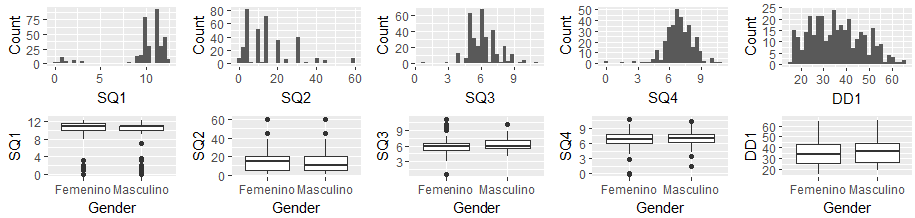
\includegraphics[width=0.9\linewidth]{images/hist-boxplots-continuous-variables} 

}

\caption{Histograms and boxplots of the continuous features}\label{fig:hb-of-cf}
\end{figure}

The plots in the Fig. \ref{fig:hb-of-cf} shows that the continuous
features have outliers which should be analyzed to include/exclude from
de dataset before of the training of the model to obtain better results.
These variables do not intervene directly in the generation of the
model, the model is generated from the SH features, however, these
outliers could be indicators of some disorder of sleep in the
respondent, thus the analysis must be performed.

The Table \ref{tab-data-quality-plan-continuous} summarizes the data
quality issues in continuous features and the potential strategies to
attend them.

\begin{table}[ht]
\centering
\caption{Data quality plan for continuous features}
\label{tab-data-quality-plan-continuous}
\begin{tabular}{|l|p{5cm}|p{8cm}|}
\hline
Feature & Data quality issue  & Strategie \\ \hline
SQ1     & Data contain 0.0, the correct value should be 12.00 & Refine the process of convert data for this field  \\ \hline
SQ4     & Data contain negative values, it is wrong because the data represents the time to wake up & Refine the process validating the data, to correct the problem, or, eliminate the records with this issue. \\ \hline
SQ2     & Standar deviation too large & Finding outliers visually and analytically. Excluding outliers from the modeling may improve the predictions. These analysis of outliers includes all continuous variables.  \\ \hline
All     & Missing values  & The percentage of missing values is low, it allows to eliminate records with missing values. The decision of impute data is a few probable, since no reports are in our bibliography to know the tendency of the data. \\ \hline
\end{tabular}
\end{table}

\section{Categorical Features for demographics
data}\label{categorical-features-for-demographics-data}

The categorical features were divided in two groups, the demographic
features are in the first group and the features containing all the
information over the sleep hygiene are in other group.

\begin{table}[ht]
\centering
\caption{Data quality report of continuous features}
\label{Report-of-quality-of-the-categorical-demographic-features}
\begin{tabular}{llllp{2cm}llp{2cm}ll}
\hline
\textbf{Feat.} & \textbf{Count} & \textbf{Miss} & \textbf{Card} & \textbf{Mode}         & \textbf{MF} & \textbf{M\%} & \textbf{Mode2} & \textbf{M2F} & \textbf{M2\%} \\ \hline
DD2              & 338            & 0             & 2             & Femenino              & 188               & 55.62\%           & Masculino      & 150                & 44.38\%            \\
DD3              & 338            & 1             & 5             & Docente               & 143               & 42.31\%           & Empleado       & 70                 & 20.71\%            \\
DD4              & 338            & 0             & 4             & Más mental que físico & 156               & 46.15\%           & Mental         & 143                & 42.31\%            \\
DD5              & 338            & 2             & 5             & ASD                   & 150               & 44.38\%           & Católica       & 129                & 38.17\%            \\
DD6              & 338            & 0             & 1             & Unión Libre           & 338               & 100\%             & NA             & NA                 & NA\%               \\
DD7              & 338            & 0             & 5             & Ninguno               & 284               & 84.02\%           & Otro           & 26                 & 7.69\%             \\
DD8              & 338            & 1             & 5             & No                    & 272               & 80.47\%           & Otra           & 34                 & 10.06\%            \\ \hline
\end{tabular}
\end{table}

The table
\ref{Report-of-quality-of-the-categorical-demographic-features} shows
only one irregularity in this set of variables, the variable DD6 has the
hihest mode posible (\(100\%\)), if data are right, all respondents are
living in free union status which is very doubtful taken in account the
population were the questionnaire was applied. There are less missing
values than in the continuous features, so, it is possible to think in
eliminate the records. The cardinality is not a problem in this set of
features (except for the variable DD6 as commented above), since all
posibilities have representation. In the two cases (features DD7 and
DD8) where the mode capture a high percentage of the data, the
information is good for this research. DD7 refers to people who suffer
some chronic disease, the best answer to this work is ``Any'' because
the intention is to work with healthy people, likewise in the DD8
variable that ask to the people if they are in some crisis that disrups
their sleep, the best answer to this work is ``No'', fortunatelly, this
is the mode.

\subsection{Categorical features for Slepp
hygiene}\label{categorical-features-for-slepp-hygiene}

\begin{table}[ht]
\centering
\caption{Report of quality of the SH features}
\label{tab:report-of-quality-of-the-sleep-hygiene-features}
\begin{tabular}{llllllllll}
\hline
\multicolumn{1}{c}{\textbf{Feature}} & \multicolumn{1}{c}{\textbf{Count}} & \multicolumn{1}{c}{\textbf{Miss}} & \multicolumn{1}{c}{\textbf{Card}} & \multicolumn{1}{c}{\textbf{Mode}} & \multicolumn{1}{c}{\textbf{MF}} & \multicolumn{1}{c}{\textbf{M\%}} & \multicolumn{1}{c}{\textbf{Mode2}} & \multicolumn{1}{c}{\textbf{M2F}} & \multicolumn{1}{c}{\textbf{M2\%}} \\
\hline
SH1    & 338    & 0   & 5  & 1     & 114   & 33.73\%   & 0   & 111  & 32.84\%  \\
SH4    & 338    & 1   & 5  & 0     & 204   & 60.36\%   & 1   & 67   & 19.82\%  \\
SH5    & 338    & 0   & 5  & 0     & 176   & 52.07\%   & 2   & 64   & 18.93\%  \\
SH6    & 338    & 1   & 5  & 0     & 152   & 44.97\%   & 1   & 75   & 22.19\%  \\
SH7    & 338    & 2   & 5  & 0     & 142   & 42.01\%   & 1   & 107  & 31.66\%  \\
SH8    & 338    & 0   & 5  & 0     & 319   & 94.38\%   & 4   & 7    & 2.07\%   \\
SH9    & 338    & 0   & 4  & 0     & 276   & 81.66\%   & 1   & 34   & 10.06\%  \\
SH10   & 338    & 0   & 5  & 0     & 223   & 65.98\%   & 1   & 57   & 16.86\%  \\
SH11   & 338    & 1   & 5  & 0     & 104   & 30.77\%   & 2   & 78   & 23.08\%  \\
SH12   & 338    & 0   & 5  & 1     & 133   & 39.35\%   & 2   & 114  & 33.73\%  \\
SH13   & 338    & 0   & 5  & 2     & 92    & 27.22\%   & 1   & 76   & 22.49\%  \\
SH14   & 338    & 0   & 5  & 0     & 210   & 62.13\%   & 1   & 61   & 18.05\%  \\
SH15   & 338    & 1   & 5  & 0     & 101   & 29.88\%   & 1   & 91   & 26.92\%  \\
SH16   & 338    & 0   & 5  & 0     & 163   & 48.22\%   & 1   & 84   & 24.85\%  \\
SH17   & 338    & 1   & 5  & 0     & 222   & 65.68\%   & 1   & 82   & 24.26\%  \\
SH18   & 338    & 0   & 5  & 0     & 173   & 51.18\%   & 1   & 82   & 24.26\%  \\
SH19   & 338    & 0   & 5  & 0     & 125   & 36.98\%   & 1   & 81   & 23.96\%  \\
SH20   & 338    & 0   & 5  & 2     & 117   & 34.62\%   & 1   & 90   & 26.63\%  \\
SH21   & 338    & 0   & 5  & 1     & 130   & 38.46\%   & 2   & 96   & 28.40\%  \\ 
\hline
\end{tabular}
\end{table}

In Table \ref{tab:report-of-quality-of-the-sleep-hygiene-features}, the
cardinality shows that all possible value \([0-5]\) for each answer is
represented in the data, except by the SH9 variable where one of the
options was not selected as answer of the respondents. It is good for
the quality of data, however, there are two variables with high mode.
The 81.66 \% of the respondents, answered \emph{never (\(0\))} to the
question SH9 \emph{``I use alcohol within 4 hours of going to bed or
after going to bed.''}, while the 94.38\% answered \emph{never (\(0\))}
to the question SH8 \emph{``I use tobacco within 4 hours of going to bed
or after going to bed.''}, which means that there are few variability in
the data in these two variables. It is possible to dispense with these
data for the analysis, since they do not contribute much information to
the studied phenomenon for this population. The other 19 categorical
variables for SHI, have a cardinality of 5, and the higher mode is
placed in SH10 \emph{``I use cafeine within 4 hours of going to bed or
after going to bed.''} were a \(66.98\%\) of the respondents answered
\emph{never (\(0\))} for this question. This means that the answers have
a good range of variability to be analized, and to participate as
candidate of be selected as feature to training the model.

This set of data has small number of missing values, however, in this
case it is possible to impute data due to the features together
represents a behavior of the person. Algorithms as KNN or a multiple
logistic regression can performs data imputation to have a good
approximation to the true data. The table
\ref{Tab:Potential-strategies-to-attend-SH-features} present the summary
of the issues and potential strategies for the SH features.

\begin{table}[ht]
\centering
\caption{Potential strategies to attend SH features}
\label{Tab:Potential-strategies-to-attend-SH-features}
\begin{tabular}{|l|p{4cm}|p{8cm}|}
\hline
Feature & Data quality issue  & Strategie  \\ 
\hline
SH8 & The mode is very high (\textgreater94\%) & Analyze the relevance of include this variable to the analysis due the few variability   \\ 
\hline
SH9 & The mode is high (\textgreater81\%)      & Analyze the relevance of include this variable to the analysis due the few variability \\ 
\hline
All & Missing values                           & The percentage of missing values is small, however, imputation will be performed for this missing values. \\ 
\hline
\end{tabular}
\end{table}

\section{Following the quality plan to attend
issues}\label{following-the-quality-plan-to-attend-issues}

The first step in order to attend the issues was the analysis of the
code that validates the raw data, to avoid the suspicious of bugs that
could be generate wrong data. After the code is validated, the errors in
data can be adjudicate to human capture.

After the analysis of scripts, tree bugs were fixed. The first bug is
related with the reason that the civil status have a mode equivalent to
the number of records in the dataset. The bug was generated by
omittining a condition in the evaluation of a missing value in the field
in the same line of code that attempt to standardize the results so that
all the sentences were in the same style of case. In the case of status
civil feature, some answers are wroten as \emph{`Unión libre'}, while
other was wroten as \emph{`Unión Libre'}.

The line with the bug:

\texttt{ifelse(is.na(dataSet\$DD6),dataSet\$DD6\textless{}-NA,dataSet\$DD6\textless{}-"Unión\ Libre")}

The line after being fixed:

\texttt{ifelse(is.na(dataSet\$DD6),dataSet\$DD6\textless{}-NA,dataSet{[}dataSet\$DD6==\textquotesingle{}Unión\ libre\textquotesingle{},7{]}\textless{}-"Unión\ Libre")}

The second bug was identified in the script that calculates the time of
sleep depending of the three variables, \emph{`Time to go the bed'},
\emph{`Time to wake up'}, \emph{`Time to fall asleep'}, in this case,
the condition for the calculation does not contemplate that a person
could say that he went to bed and got up twelve hours apart. The problem
was solved by modifying the conditional operator of \(>\) to \(\geq\).

Code with bug:

\begin{verbatim}
  if(HD>HL){
    HD<-HD-12.00
  }
  SE<-abs(HL-HD)
  SE<-SE-round(minutos/60,digits = 2)
\end{verbatim}

Code after being fixed:

\begin{verbatim}
  if(HD>=HL){
    HD<-HD-12.00
  }
  SE<-abs(HL-HD)
  SE<-SE-round(minutos/60,digits = 2)
\end{verbatim}

The third bug was corrected by adding two condition per values before
ignored. Values in the range of \((-\infty,0)\) must be taken a NA
value, and values in the range of \([0,1)\) must be transformed by
adding 12.00.

The lines that were added are:

\begin{verbatim}
  if(!is.na(s3)){
    if(as.numeric(s3)<0){
      s3<-NA
    }else if(as.numeric(s3)<1){
      s3=as.numeric(s3)+12
    }else{
      s3<-as.numeric(s3)
    }
  }
\end{verbatim}

The quality reports generated after apply this corrections, show a
difference in the identified features with possible issues due to a
wrong treatment.

\begin{table}[ht]
\centering
\caption{Quality report of continuous features after recoding the scripts}
\label{tab-quality-report-continuous-after-recoding-scripts}
\begin{tabular}{lllllllllll}
\hline
\multicolumn{1}{c}{\textbf{Feature}} & \multicolumn{1}{c}{\textbf{Count}} & \multicolumn{1}{c}{\textbf{Miss}} & \multicolumn{1}{c}{\textbf{Card}} & \multicolumn{1}{c}{\textbf{Min}} & \multicolumn{1}{c}{\textbf{Qrt1}} & \multicolumn{1}{c}{\textbf{Median}} & \multicolumn{1}{c}{\textbf{Qrt3}} & \multicolumn{1}{c}{\textbf{Max}} & \multicolumn{1}{c}{\textbf{Mean}} & \multicolumn{1}{c}{\textbf{Sdev}} \\ 
\hline
DD1   & 338  & 6  & 49  & 16  & 27    & 35  & 44    & 66    & 35.92    & 11.41     \\
SQ1   & 338  & 0  & 27  & 1   & 10    & 11  & 11.5  & 12.75 & 10.17    & 2.46      \\
SQ2   & 338  & 1  & 15  & 1   & 5     & 15  & 20    & 60    & 14.99    & 11.91     \\
SQ3   & 338  & 2  & 40  & 3   & 5.21  & 6   & 7     & 12.7  & 6.21     & 1.33      \\
SQ4   & 338  & 3  & 107 & 0.12& 6.17  & 6.89& 7.75  & 11.95 & 6.94     & 1.33      \\ 
\hline
\end{tabular}
\end{table}

\begin{table}[ht]
\centering
\caption{Quality report of demographic features after recoding the scripts}
\label{tab-quality-report-demographic-after-recoding-scripts}
\begin{tabular}{llllp{2cm}lllll}
\hline
\multicolumn{1}{c}{\textbf{Feature}} & \multicolumn{1}{c}{\textbf{Count}} & \multicolumn{1}{c}{\textbf{Miss}} & \multicolumn{1}{c}{\textbf{Card}} & \multicolumn{1}{c}{\textbf{Mode}} & \multicolumn{1}{c}{\textbf{MF}} & \multicolumn{1}{c}{\textbf{M\%}} & \multicolumn{1}{c}{\textbf{Mode2}} & \multicolumn{1}{c}{\textbf{M2F}} & \multicolumn{1}{c}{\textbf{M2\%}} \\ \hline
DD2   & 338  & 0   & 2    & Femenino                  & 188   & 55.62\%  & Masculino      & 150  & 44.38\%  \\
DD3   & 338  & 1   & 5    & Docente                   & 143   & 42.31\%  & Empleado       & 70   & 20.71\%  \\
DD4   & 338  & 0   & 4    & Más mental que físico     & 156   & 46.15\%  & Mental         & 143  & 42.31\%  \\
DD5   & 338  & 2   & 5    & ASD                       & 150   & 44.38\%  & Católica       & 129  & 38.17\%  \\
DD6   & 338  & 0   & 5    & Casada(o)                 & 181   & 53.55\%  & Soltera(o)     & 119  & 35.21\%  \\
DD7   & 338  & 0   & 5    & Ninguno                   & 284   & 84.02\%  & Otro           & 26   & 7.69\%   \\
DD8   & 338  & 1   & 5    & No                        & 272   & 80.47\%  & Otra           & 34   & 10.06\%  \\ \hline
\end{tabular}
\end{table}

The minimum value in SQ1 is not zero as before, now it is one, which is
reasonable; the variable SQ4 do not have a negative value as minimum
value. The present also is very small (\(0.12\)) and was verified in the
raw data, the conclusion is that it was a wrong user capture, the
respondent said that he/she go to bed at 12:30 and wakes up at 12:42
every day. On the other hand, the civil status (DD6) has a congruent
value for the sample of study, the \(53.55\%\) of the respondents said
be married and \(35.21\%\) be single, in contrast with previous data
where it was reported that \(100\%\) of the people had a `Free union'
civil status.

The second step was to work with the missing values in the continuous
features and missing values in the categorical demographic features.
Records containing missing values were eliminated as proposed in the
data qulaity plan described in Table
\ref{tab-data-quality-plan-continuous}. The same apply to the
categorical demographic features.

After applying the process to delete records with missing values in
continuous and categorical demographics features the dataset reducts its
dimentionality from 338 to 326, which represents a reduction of 0.036\%
of the original data.

In the third step of this stage the atypical values are identified to
exclude them from the dataset that will serve as a source of the
training of the model. The process excludes records that exceed three
standard deviations in the variable SQ4 (`time the person spent
asleep'). This variable is of high impact on the quality of sleep and is
not considered within the factors of sleep hygiene. Another indicator of
a possible sleep disorder is the latency, latency is the time between a
person go to bed and he/she fall asleep. The records containing outliers
in this feature, also were eliminated.

After delete records with outliers n continuous variables the dataset
reducts its dimentionality from 338 to 306, which represents a reduction
of 0.095\% of the original data.

The Fig. \ref{fig:hb-of-cf-after-deloutliers}, shows the histograms and
boxplots after eliminated records with outliers in SQ2 and SQ4, boxplots
in these two variables make it clear that do not outliers were found for
these features. DD1 has no outliers too, even though maintaining the
original records.

\begin{figure}[H]

{\centering 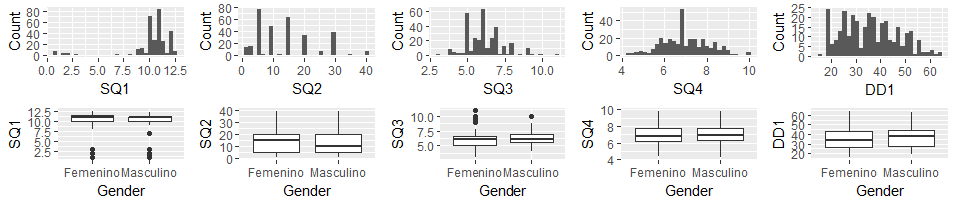
\includegraphics[width=0.9\linewidth]{images/hist-boxplots-continuous-variables-after-delete-outliers} 

}

\caption{Histograms and boxplots of the continuous features after delete outliers}\label{fig:hb-of-cf-after-deloutliers}
\end{figure}

\section{Imputation of missing values in SH and SQ
features}\label{imputation-of-missing-values-in-sh-and-sq-features}

The process of imputation was performed using \emph{mice and VIM
package} \citep[\citet{VIM2016}]{mice2011}. the process begins with the
analysis of missing values in the variables involved indirectly or
directly in the generation of the model. The table
\ref{tab-report-of-missing-value-in-SHSQ} shows that the dataset has few
missing values (Not all columns in the table are included for lack of
space, however, all columns that were omitted do not have missing
values). It has \(297\) complete records, a record with a missing value
in the column SQ5a, one more with a missing value in the column SQ5c, an
so on. The dataset contains eight records with a total of nine missing
values in eight variables.

\begin{table}[ht]
\centering
\caption{Report of missing values}
\label{tab-report-of-missing-value-in-SHSQ}
\begin{tabular}{|l|l|l|l|l|l|l|l|l|l|l|l|l|l|l|}
\hline
    & SQ5b & SQ5d & ... & SH20 & SH21 & SQ5a & SQ5c & SH4 & SH6 & SH11 & SH15 & SH17 & SH7 &   \\ \hline
297 & 1    & 1    & ... & 1    & 1    & 1    & 1    & 1   & 1   & 1    & 1    & 1    & 1   & 0 \\ \hline
1   & 1    & 1    & ... & 1    & 1    & 0    & 1    & 1   & 1   & 1    & 1    & 1    & 1   & 1 \\ \hline
1   & 1    & 1    & ... & 1    & 1    & 1    & 0    & 1   & 1   & 1    & 1    & 1    & 1   & 1 \\ \hline
1   & 1    & 1    & ... & 1    & 1    & 1    & 1    & 0   & 1   & 1    & 1    & 1    & 1   & 1 \\ \hline
1   & 1    & 1    & ... & 1    & 1    & 1    & 1    & 1   & 0   & 1    & 1    & 1    & 1   & 1 \\ \hline
2   & 1    & 1    & ... & 1    & 1    & 1    & 1    & 1   & 1   & 1    & 1    & 1    & 0   & 1 \\ \hline
1   & 1    & 1    & ... & 1    & 1    & 1    & 1    & 1   & 1   & 0    & 1    & 1    & 1   & 1 \\ \hline
1   & 1    & 1    & ... & 1    & 1    & 1    & 1    & 1   & 1   & 1    & 0    & 1    & 1   & 1 \\ \hline
1   & 1    & 1    & ... & 1    & 1    & 1    & 1    & 1   & 1   & 1    & 1    & 0    & 1   & 1 \\ \hline
    & 0    & 0    & ... & 0    & 0    & 1    & 1    & 1   & 1   & 1    & 1    & 1    & 2   & 9 \\ \hline
\end{tabular}
\end{table}

A summary of the missing values its presented in the table
\ref{summary-of-missing-values-SH}

\begin{table}[ht]
\centering
\caption{Summary of missing values in SH features}
\label{summary-of-missing-values-SH}
\begin{tabular}{|l|l|}
\hline
Feature & Count of missing values \\ \hline
SQ5a    & 1                       \\ \hline
SQ5b    & 1                       \\ \hline
SH4     & 1                       \\ \hline
SH6     & 1                       \\ \hline
SH7     & 2                       \\ \hline
SH11    & 1                       \\ \hline
SH15    & 1                       \\ \hline
SH17    & 1                       \\ \hline
Total   & 7                       \\ \hline
\end{tabular}
\end{table}

The figure \ref{fig:f-pattern-of-missing-data} shows in the left side,
an histogram of the features with missing data depicting the influence
of missing values in the dataset. The right side shows the pattern of
missing values in the dataset, it concentrates all complete cases in the
botton of the graph, which reach a 97.06\% of the dataset. The remaining
of the figure shows the features with missing data, placing in the right
side the corresponding percentages per variable.

\begin{figure}[H]

{\centering 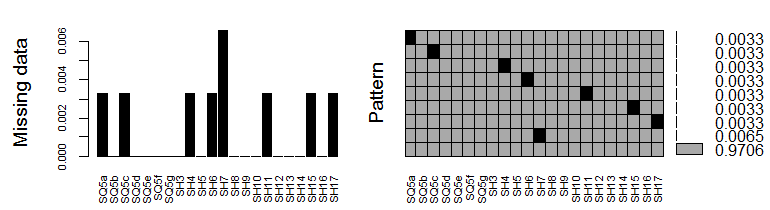
\includegraphics[width=0.9\linewidth]{images/pattern-of-missing-data} 

}

\caption{Pattern of missing values}\label{fig:f-pattern-of-missing-data}
\end{figure}

The \emph{mice} function was executed to impute data in the records
containing missing values, the process was performed in a temporal
dataset comformed only for those features with missing data. The
\emph{mice} function perform data imputation using \emph{polytomous
regression imputataion} for unordered categorical data with more of two
leves, which is the case. The multinomial logistic regression was
applied with 50 iterations and five datasets to obtain a table of
results that allow to choose the best option to do the imputation.

\begin{table}[ht]
\centering
\caption{Five datasets with data imputation}
\label{datasets-of-impute-data}
\begin{tabular}{|l|l|l|l|l|l|}
\hline
Number of Row & DS1 & DS2 & DS3 & DS4 & DS5 \\ \hline
ROW 225       & 2   & 1   & 0   & 1   & 3   \\ \hline
ROW 72        & 3   & 1   & 0   & 2   & 2   \\ \hline
ROW 12        & 0   & 0   & 0   & 0   & 3   \\ \hline
ROW 233       & 2   & 1   & 1   & 4   & 2   \\ \hline
ROW 17        & 0   & 1   & 2   & 1   & 0   \\ \hline
ROW 146       & 0   & 1   & 2   & 0   & 2   \\ \hline
ROW 144       & 3   & 0   & 0   & 3   & 1   \\ \hline
ROW 183       & 0   & 4   & 0   & 3   & 4   \\ \hline
ROW 201       & 0   & 2   & 0   & 0   & 0   \\ \hline
\end{tabular}
\end{table}

The DS4 is the dataset most consistent with the proposals in the other
datasets, it matches with at least one dataset of the remaining four, in
seven of the rows. The DS4 was chosen to impute data in these variables.

\begin{table}[ht]
\centering
\caption{Report of missin gvalues after imputation}
\label{tab-report-of-missingvalues-after-imputation}
\begin{tabular}{lllllllll}
SQ5a & SQ5c & SH4 & SH6 & SH11 & SH15 & SH17 & SH7 &   \\
1    & 1    & 1   & 1   & 1    & 1    & 1    & 1   & 0 \\
0    & 0    & 0   & 0   & 0    & 0    & 0    & 0   & 0
\end{tabular}
\end{table}

The table \ref{tab-report-of-missingvalues-after-imputation}, shows that
no missing value are in the dataset after the imputation, now the new
dataset of variables with data imputation will be merged with the others
features of the original dataset in a new dataset to be saved and used
in advanced to train the model.

\section{Final results}\label{final-results}

The following tables show the report of quality in the dataset after
apply deletion of missing values, exclusion of records containing
outliers and imputation of missing values in variables that are closely
related with the training of the model.

\begin{table}[ht]
\centering
\caption{Report of Quality of SH features after cleaning and imputation}
\label{tab-report-of-quality-of-sh-features}
\begin{tabular}{|l|l|l|l|l|l|l|l|l|l|}
\hline
Feature & Count & Miss & Card & Mode & ModeFrec & ModePerc & Mode2 & Mode2Frec & Mode2Perc \\ \hline
SH1     & 306   & 0    & 5    & 1    & 109      & 35.62\%  & 0     & 97        & 31.70\%   \\ \hline
SH2     & 306   & 0    & 5    & 1    & 109      & 35.62\%  & 2     & 107       & 34.97\%   \\ \hline
SH3     & 306   & 0    & 5    & 1    & 147      & 48.04\%  & 2     & 70        & 22.88\%   \\ \hline
SH4     & 306   & 0    & 5    & 0    & 186      & 60.78\%  & 1     & 63        & 20.59\%   \\ \hline
SH5     & 306   & 0    & 5    & 0    & 159      & 51.96\%  & 2     & 56        & 18.30\%   \\ \hline
SH6     & 306   & 0    & 5    & 0    & 135      & 44.12\%  & 1     & 69        & 22.55\%   \\ \hline
SH7     & 306   & 0    & 5    & 0    & 128      & 41.83\%  & 1     & 99        & 32.35\%   \\ \hline
SH8     & 306   & 0    & 5    & 0    & 292      & 95.42\%  & 3     & 5         & 1.63\%    \\ \hline
SH9     & 306   & 0    & 4    & 0    & 254      & 83.01\%  & 1     & 30        & 9.80\%    \\ \hline
SH10    & 306   & 0    & 5    & 0    & 201      & 65.69\%  & 1     & 53        & 17.32\%   \\ \hline
SH11    & 306   & 0    & 5    & 0    & 95       & 31.05\%  & 2     & 69        & 22.55\%   \\ \hline
SH12    & 306   & 0    & 5    & 1    & 122      & 39.87\%  & 2     & 99        & 32.35\%   \\ \hline
SH13    & 306   & 0    & 5    & 2    & 85       & 27.78\%  & 1     & 69        & 22.55\%   \\ \hline
SH14    & 306   & 0    & 5    & 0    & 188      & 61.44\%  & 1     & 54        & 17.65\%   \\ \hline
SH15    & 306   & 0    & 5    & 0    & 94       & 30.72\%  & 1     & 80        & 26.14\%   \\ \hline
SH16    & 306   & 0    & 5    & 0    & 150      & 49.02\%  & 1     & 76        & 24.84\%   \\ \hline
SH17    & 306   & 0    & 5    & 0    & 200      & 65.36\%  & 1     & 78        & 25.49\%   \\ \hline
SH18    & 306   & 0    & 5    & 0    & 158      & 51.63\%  & 1     & 73        & 23.86\%   \\ \hline
SH19    & 306   & 0    & 5    & 0    & 112      & 36.60\%  & 1     & 78        & 25.49\%   \\ \hline
SH20    & 306   & 0    & 5    & 2    & 107      & 34.97\%  & 1     & 85        & 27.78\%   \\ \hline
SH21    & 306   & 0    & 5    & 1    & 122      & 39.87\%  & 2     & 88        & 28.76\%   \\ \hline
\end{tabular}
\end{table}

With exception of high percentages in mode of the SH8 and SH9, all other
features present a good behavior in the dataset. The issue of SH8 and
SH9 will be attended in a future stage of the work, the process of
feature selection will take care of this.

The last process to be carried out in this stage is the calculation of
SHI and PSQI scores through the scales provided by the respective
questionnaires.

The final dataset to be used in the process of feature selection is a
306 x 62 dataset containing 10 continuous features, 51 categorical
features and one ID feature. To more detail of this dataset, see please
the tables at the end of the previous section.

\hypertarget{feature-selection}{\chapter{\texorpdfstring{\protect\hyperlink{feature-selection}{Feature
selection}}{Feature selection}}\label{feature-selection}}

This section describes the process that we perform to reduce the
dimension of the sleep hygiene data set that contains the features to
model the quality of sleep for respondents of the survey described in
chapter \ref{data-adquisition}. There exist two ways to addressed
dimensionality reduction, feature extraction and feature selection.
Feature extraction, consists in generate a new and small feature space.
The application of a technique of feature extraction produce new
features based in original ones. The new dataset is not understandable
in terms of the original dataset, rather, it is an abstraction of this
and its visualization have no practical meaning. On the other hand,
feature selection as ilustrate the Fig.
\ref{fig:feature-selection-process} choose a small subset of the
relevant features from the original dataset according to certain
relevance evaluation criterion, which usually leads to better learning
performance, lower computational cost, and better model interpretability
\citep{Tang2014}.

\begin{figure}[H]

{\centering 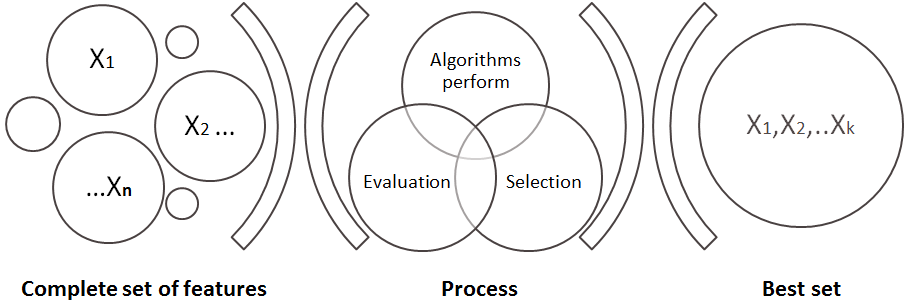
\includegraphics[width=0.8\linewidth]{images/feature-selection-process} 

}

\caption{Feature selection Process}\label{fig:feature-selection-process}
\end{figure}

For the purposes of this study, the technique of selection of
characteristics is the most appropriate. Our interest in reducing
dimensionality is not related to the decrease in computational cost,
rather, the purpose is to decrease the number of predictive variables
due to the high cost of design and infrastructure that means capturing
21 different signals through sensors. If it is possible to characterize
a high percentage of the phenomenon, through a reduced number of factors
of sleep hygiene, the design of the system will be more feasible and
less expensive.

The model accuracy for prediction of the sleep quality with the subset
of features must be better than the training model using the total of
sleep hygiene features.

\section{\texorpdfstring{\protect\hyperlink{feature-selection-model}{Feature
selection
models}}{Feature selection models}}\label{feature-selection-models}

In 1996, \citep{Liu1998} proposes two models to achieve the reduction of
features, that have been used as basis of diverse algorithms still in
force. The filter model (see Figure \ref{fig:filter-model}) that uses as
criterion of feature selection, some attributes concerning only to the
data domain. Especifiacally in this model, Liu et. al. proposes that it
is posible to analyze and make decisions over irrelevance or relevance
of features based in measure information gain, dependence, distance and
consistency.

\begin{figure}[H]

{\centering 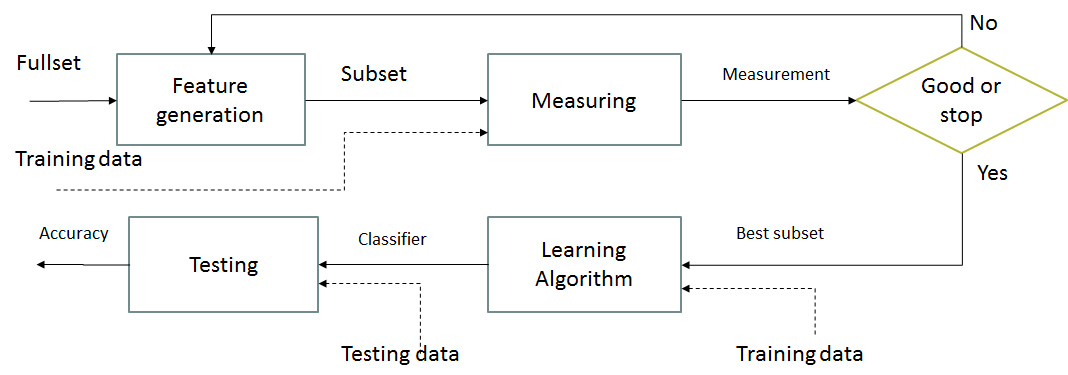
\includegraphics[width=0.6\linewidth]{images/filter-model} 

}

\caption{Filter model proposed by Liu et. al.}\label{fig:filter-model}
\end{figure}

The second model showed in Fig. \ref{fig:wrapper-model} proposed is the
wrapper model that uses the accuracy of prediction as selection
criterion, it means that this techniques are committed with a particular
classifier in this stage of the learning process.

\begin{figure}[H]

{\centering 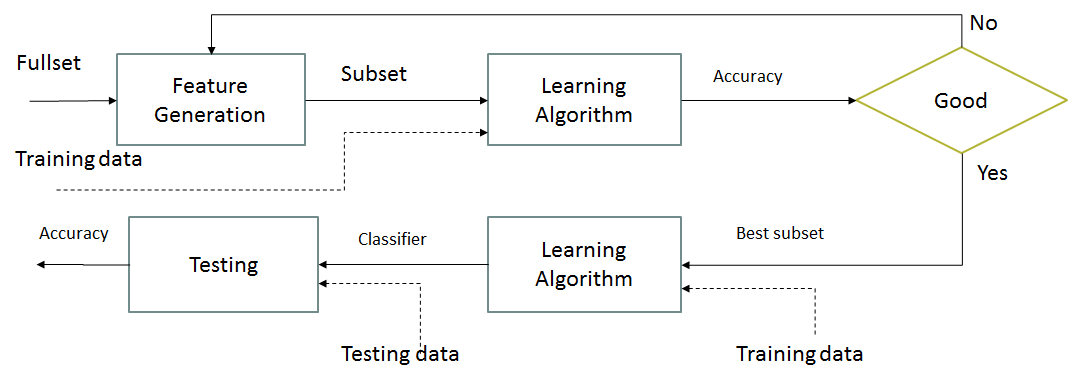
\includegraphics[width=0.6\linewidth]{images/wrapper-model} 

}

\caption{Wrapper model proposed by Liu et. al.}\label{fig:wrapper-model}
\end{figure}

Both models have advanteges and disadvantages, techniques based in
filter model, performs better than others based in wrapper model,
however, researchers have no idea over prediction accuracy during the
feature selection process. Some practitioners don't preffer to use these
techniques because if accuracy prediction is not achieved in the
proposed level, the first steep can be regarded as a waste of time. On
the other hand, some researchers argued that select features based in
determinated classifier, reduces the possibility to use other classifier
to generate the prediction model, in this sense, the classifier to
generate the final model should be choosed at the begining, and it is
not convenient for all problems. In these order of thinks,
\citep{Kelleher2015} comment that wrapper models are more
computationally expensive than filters models and that the argument of
they are uncertain models respect to the accuracy, is not at all valid
since filters model often generate models with good accuracy.

Additionaly, \citep{Liu1998} highlight \emph{Search}, \emph{Scheme} and
\emph{measure} as three important concepts that help to decide what
technique is the most appropriate for an specific problem of
dimentionality reduction by feature selection (see Fig.
\ref{fig:main-dimensions-dr}). Search refers to the activity of choose
features in non deterministic, heuristic or complete form, Scheme must
be determine if the search will be forward, backward or in random mode,
and, measure has to do with tree ways to establish the threshold for
stopping the feature search, the criterion used are accuracy,
consistency, and, classic criterion involving distance, information gain
and dependence.

\begin{figure}[H]

{\centering 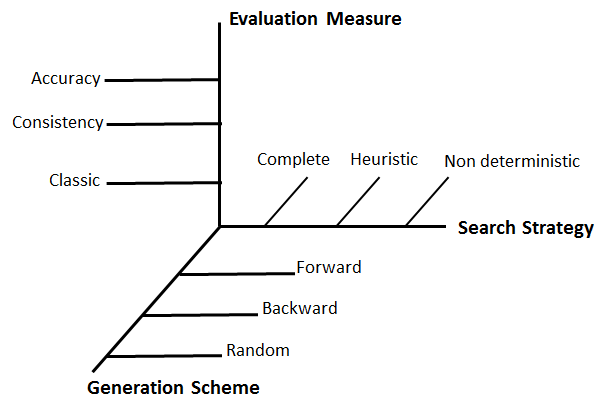
\includegraphics[width=0.6\linewidth]{images/main-dimensions-in-feature-selection} 

}

\caption{Main dimensions in feature selection, Liu et. al.}\label{fig:main-dimensions-dr}
\end{figure}

A third type of model has been proposed in last years, these models are
called \textbf{embedded models}, since they allow practitoners select
features while the prediction model is built. Embedded models have the
advantage of filters model in terms of low computational cost, and take
the advantage of wrapper model, because the prediction accuracy and
classification model are involved in the process. \citep{Tang2014}
describe three type of embedded methods as we shows in the Table
\ref{tab:table-embedded-methods}.

\begin{table}[h]
\centering
\caption{Embedded methods as \cite{Tang2014} describes and quoted verbatim in his paper.}
\label{tab:table-embedded-methods}
\begin{tabular}{|>{\centering\arraybackslash}p{3cm}|>{\arraybackslash}p{10cm}|>{\centering\arraybackslash}p{2cm}|}
\hline Method & Description & Cite \\ 
\hline Pruning & Utilizing all features to train a model and then attemp to eliminate some features by setting the corresponding coefficients to 0, while maintaining model performance such as recursive feature elimination using support vector machines (SVM) & \cite{Guyon2002} \\ 
\hline Build-in & Mechanism for feature selection as ID3 and C4.5 & \cite{Quinlan1986,Quinlan1993} \\ 
\hline Regularization & Utilices objective functions that minimize fitting errors and in the mean time force the coefficients to be small or ti be exact zero. & \cite{Ma2008} \\ 
\hline 
\end{tabular} 
\end{table}

These models are representative of the theoretical basis where a lot of
algorithms for selection features in last twenty years have been fueled.
Likewise four concepts are the most important and have been used for the
generation of different feature selection algorithms in last two
decades: distance, accuracy, inconsistency and information gain.

\begin{itemize}
\tightlist
\item
  Distance: The main goal to use distance, is to find similarity among
  instances in a dataset. The Equation proposed by Minkowski (see eq.
  \eqref{eq:Minkowski}) is a generalization of the distances that are used
  in MLA. The most common distances are the particular cases where
  \(p=1\) called Manhatan distance (see Eq. \eqref{eq:Manhattan}) and
  where \(p=2\), the well known Euclidian distance (see Eq.
  \eqref{eq:Euclidean}). (All three equations were taken from
  \citep{Kelleher2015}). The implication of use different values of
  \(p\) will be noted in the difference between two values of any
  feature in the final distance, it is directly proportional to the
  value of \(p\). It means that large differences between two features
  in an instance, impact stronger in the final result when \(p\) grows.
\end{itemize}

\begin{equation}
      Euclidean(A,B)=\sqrt{(a_1-b_1)^2+(a_2-b_1)^2+\dots+(a_n-b_n)^2}
      \label{eq:Euclidean}
\end{equation}

\begin{equation}
      Manhattan(a,b)=\sum_{i=1}^{m}abs(a[i]-b[i])
      \label{eq:Manhattan}
\end{equation}

\begin{equation}
    Minkowski(a,b)=\left({\sum_{i=1}^{m}abs(a[i]-b[i])^p}\right)^{\frac{1}{p}}
    \label{eq:Minkowski}
\end{equation}

\begin{itemize}
\tightlist
\item
  Accuracy: Accuracy refers to the successes that a model had to predict
  each instance of a dataset, it is opposed to the miscalssification
  error as \citep{Kelleher2015} defines in
  \eqref{eq:math-misclassification-rate} and \eqref{eq:math-accuracy}
  equations. These two equation take relevance when accuracy is analized
  in the context of confusion matrix, a tool widely used to report the
  outcomes of the prediction thorugh a model. The confusion matrix
  together with the Receiver Operating Characteristics (ROC) curve,
  provides understanding and visualization of the specificity and
  sensibility, the most important metrics for evaluations of the models,
  especially in the health context.
\end{itemize}

\begin{equation}
  misclassification\ rate=\frac{(FP+FN)}{(TP+TN+FP+FN)}
  \label{eq:math-misclassification-rate}
\end{equation}

\begin{equation}
  accuracy=\frac{(TP+TN)}{(TP+TN+FP+FN)}
  \label{eq:math-accuracy}
\end{equation}

\begin{itemize}
\item
  Inconsistency: An inconsistency refers that two instances have the
  same value in all descriptive features, but they belong to a different
  class. We can compute two values to measure the inconsistency for a
  subset of features in a dataset. The first value, which is called the
  inconsistency count (\(IC\)), can be defined as \(IC=nM-LCI\), where
  \(nM\) is the number of instances that coincide in all descriptive
  features, and, \(LCI\) is the largest class of the clases that are
  involved in this particular group of instances. The second value, is
  the inconsistency rate defined as \(IR=\frac{\sum_{i=0}^{m}IC_i}{N}\),
  where \(m\) is the total of groups of matching instances in the
  dataset.
\item
  Information Gain: Is a measure of the relevance that a predictive
  variable offers in relation to the target variable. To understand the
  concept of information gain, it is necessary to first understand the
  concept of information entropy as was raised by Shannon in 1948. In a
  dataset, an entropy value represents the heterogenity/homogenity of
  the target variable, in others words, if we have large probability of
  success to predict an outcome in the target feature, we have a set
  with small entropy and viceversa.
\end{itemize}

The process to calculate the information gain of one feature can be
sumarized as follows:

\begin{enumerate}
\def\labelenumi{\arabic{enumi}.}
\tightlist
\item
  Compute the total entropy.
\item
  Split the target feature in the levels of the predictive feature.
\item
  Compute the entropy of the target variable in each subset generate,
  and multiply the result by its weight. The weight is computed by
  dividing the number of instances in the subset, among the total number
  of instances in the dataset.
\item
  Subtrac form the total entropy, the entropy computed in the steps
  \(2\) y \(3\).
\item
  Sort the results in descending order to identify which are the best
  and the worst features in terms of provide information to characterize
  the phenomenon.
\end{enumerate}

\section{Feature selection process}\label{feature-selection-process}

Five methods for feature selection were selected to make the process of
selection the relevant sleep hygiene factors. Each method works with the
complete set of features and the total of the data, after the process,
the features were ordered by relevance in descending order in each
method. A merge process was performed to choose those features that were
ranked in the first places in each method. This process ensure that
features choosen are relevant features because the theory and math
behind the methods are different in each one. The Fig.
\ref{fig:four-methods-of-feature-selection} shows four of the six
methods (for space reasons), and the corresponding features (Factor) and
weights (Pesos) in descending order. The Fig. \ref{fig:selected-factors}
shows the outcomes of selected factors by the merge process. The left
side, is the table with features and the corresponding weights in the
best algorithms, in these case Random Forest (RF), Logistic Regression
(LR) and Logistic Regression with Cross Validation (LR\_CV). The right
side ilustrate in a line-graph, the comparisson of the data in the table
of the left side. Both figures are screens capture of the application
developed on Shiny R-Studio for this specific purpose.

\begin{figure}[H]

{\centering 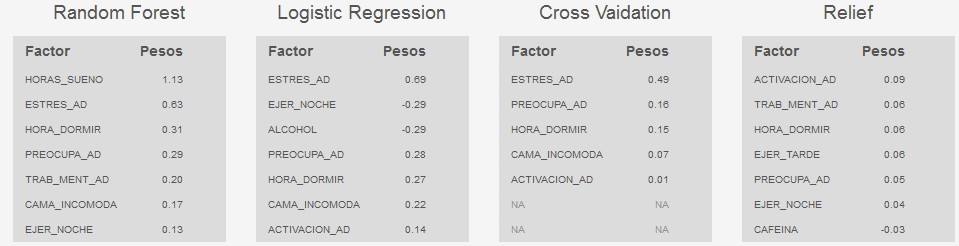
\includegraphics[width=0.8\linewidth]{images/four-methods-of-feature-selection} 

}

\caption{Results of four methods after performs Feature Selection}\label{fig:four-methods-of-feature-selection}
\end{figure}

\begin{figure}[H]

{\centering 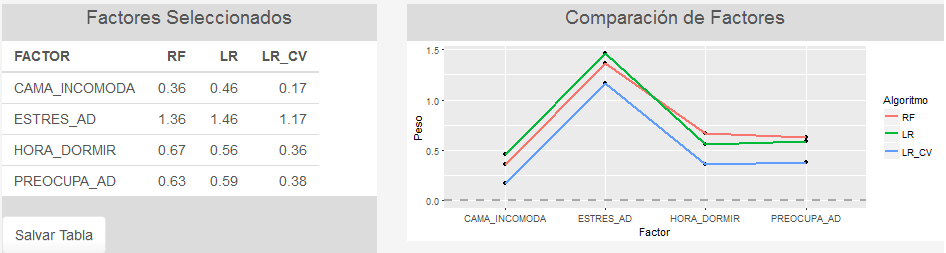
\includegraphics[width=0.8\linewidth]{images/selected-factors} 

}

\caption{Outcomes for selected factors after the merge process}\label{fig:selected-factors}
\end{figure}

From the original 21 hygiene factors that in theory are the predictive
variables to characterize the sleep quality, the feature selection
algorithms choose four features. It means that the remaining seventeen
features, there are not relevant factors to characterize the phenomenon
on this population. As additional information related with the studied
phenomenon, it is possible to note that two features closely related
with the state of mind, are present among features selected. Even, one
of this two features, the stress before go to the bed (ESTRES\_AD), is
the most relevant feature of the four selected. If this selection
provides the best model to characterize the phenomenon, a great
challenge is perceived in the near future, due to how difficult it can
be to measure a subjective variable, by means of an electronic device.

\hypertarget{evaluation-of-efficiency}{\chapter{\texorpdfstring{\protect\hyperlink{evaluation-of-efficiency}{Evaluation
of
Efficiency}}{Evaluation of Efficiency}}\label{evaluation-of-efficiency}}

Before testing the selected factors, models were trained using the 21
sleep hygiene factors to know the predictive efficiency that these
models from various techniques of machine learning could achieve. The
result was that both, the support vector machines (SVM) with linear
kernel and logistic regression, were the two techniques with the best
results. The SVM algorithm had an efficiency of 67\% and the logistic
regression reached an efficiency of 70\%. With this background, the
tests described below were made, taking into account only the four
selected factors. If any of the techniques reaches an efficiency equal
to or higher than the previous results, the selection of variables can
be considered a successful process and these factors will be used for
the prediction model of the study hereafter.

One of the steps in the development of the investigation project,
includes the selection of a technique to train a predictive model on
supervised automated learning. We did a review of the literature and we
select three techniques under certain criterion based in the nature of
the problem. The purpose is train the model with the available data and
select the one given the best prediction. So, at the same time that the
evaluation of efficience of the selected factors was performed, the
selection of the technique that will be used for the final training was
done. The three techniques that meet the inclusion criteria, were:
artificial neural networks, vector supported machines And logistic
regression with regularization. As in feature selection, a Shiny
application was developed to process the data and compare the outcomes
for these three algorithms, training a model with total of the records
and only the four features selected in the feature selection process as
was explained in Section \ref{feature-selection}.

The evaluation was performed by the cross validation technique using an
iteration process of training, validation, analysis and refinement as
the figure \ref{fig:cross-validation-process} shows. In this process a
sixty percent of the data was used to train the model, when training
conclude, the cross validation is performed through the prediction of
the target variable in the cross validation set, containing a twenty
percent of the main dataset. The analysis is done at that time and
depending on the results, the parameters are adjusted to make a new
iteration or reach the stop point. If the stop point was reached, the
model is proved in the test set to obtain the final efficience of the
model.

\begin{figure}[H]

{\centering 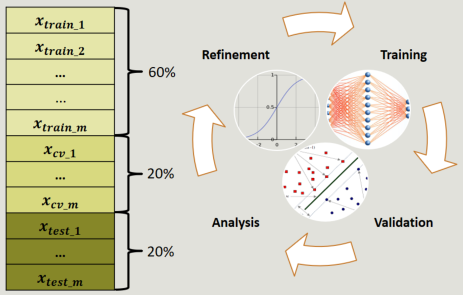
\includegraphics[width=0.8\linewidth]{images/cross-validation-process} 

}

\caption{Cross Validation Process}\label{fig:cross-validation-process}
\end{figure}

\section{\texorpdfstring{\protect\hyperlink{NN-results}{Neural Networks
Results}}{Neural Networks Results}}\label{neural-networks-results}

Two neural networks were trained and validated by cross validation
process, both estructures with a hidden layer. The first neural network
had three neurons in the hidden layer and the second four neurons. The
Fig. \ref{fig:nn-four-neurons} shows the structure of the neural network
with four neurons in the input layer, one neuron for each factor
selected in the feature selection process. The second layer is the
hidden layer with four neurons and the last layer contains one neuron
for the result (good sleep quality/bad sleep quality). Additionaly it is
possible to observe the two activation neurons in the top of the figure.

\begin{figure}[H]

{\centering 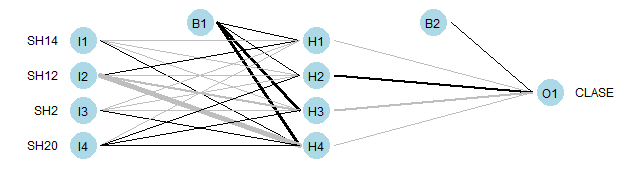
\includegraphics[width=0.8\linewidth]{images/nn-four-neurons} 

}

\caption{Structure of neural network with four neurons in the hidden layer}\label{fig:nn-four-neurons}
\end{figure}

The results for the two neural networks and the appropriate comparison
between them, are in the Fig. \ref{fig:results-of-the-3-4-nn}. The
network with better efficiency of two networks is the network with four
neurons. The table describes that in the three sets, the behavior was
superior in terms of efficiency, while the plot represents the error per
each set with three and four neurons. Clearly, the lines decrease in
favor of the training and validation with four neurons, where the error
of the prediction is smaller.

\begin{figure}[H]

{\centering 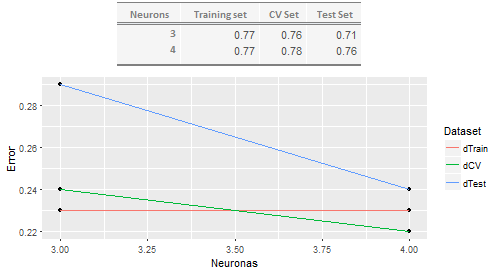
\includegraphics[width=0.8\linewidth]{images/results-of-the-3-4-nn} 

}

\caption{Comparison of the results for the two trained neural networks}\label{fig:results-of-the-3-4-nn}
\end{figure}

The results of the neural network, satisfy the conditions sought,
because although it is not greatly improved in efficiency when compared
to what can be obtained by employing all the factors of sleep hygiene,
we gain in the amount of factors that must be sensed to obtain input
data. This fact has great relevance for the project because it greatly
limits the design and infrastructure of the data acquisition module.

\section{\texorpdfstring{\protect\hyperlink{LR-results}{Logistic
Regression
Results}}{Logistic Regression Results}}\label{logistic-regression-results}

We train the model through logistic regression (LR) with regularization
parameter and polynomials of degree one, two and three, in order to look
for the optimal point between over fit and bias. The regularization
parameter based on the norm \(l_2\) takes the form of the equation
\eqref{eq:regularization-parameter}, where \(\lambda\) took values from
0.1 to 0.6 with intervals of 0.03 to choose the optimal value.

\begin{equation}
  reg=\frac{\lambda}{2m}\sum_{j=2}^{n}\theta_j^2
  \label{eq:regularization-parameter}
\end{equation}

The stop condition for the adjustment of the parameters of the
regression is of the order of one hundred thousandths, that is to say,
while the previous and the current cost function did not have a
difference of 0.00003 between both, the regression continued to iterate.

The results of LR's are shown by the application in the format of the
Fig. \ref{fig:lr-poly-1}. This figure shows the original results for the
LR with the polynomial of degree one, we obtained five coeficients
including the intercept coeficient, the right table have the data of
prediction, \(70\%\) of efficiency for the training set, \(76\%\) for
the cross validation set and \(69\%\) in the test set. The plot in the
top of figure, shows the behavior of the cost funtion through the
iterations in the compute and refinement of the parameters.

\begin{figure}[H]

{\centering 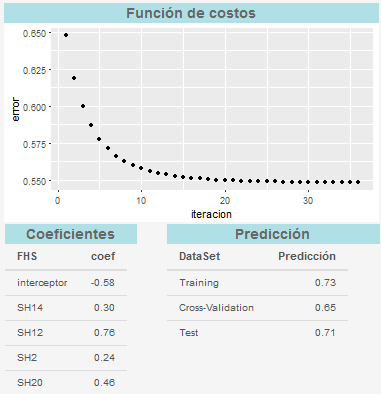
\includegraphics[width=0.8\linewidth]{images/lr-poly-1} 

}

\caption{Results of the LR and polynomial grade one}\label{fig:lr-poly-1}
\end{figure}

For polynomials of degree two and three we have a similar figure, the
difference is the number of coeficients that in the case of the
polynomial of degree two are 16 and, in the polynomial of grade three
are 35, including in both cases \emph{dummy factors}. In the case of
polynomial of degree two the cost function iterated 150 times and the
predictions were \(72\%\) of efficiency for the training set, \(78\%\)
for the cross validation set and \(69\%\) for the test set. The LR with
the polynomial of degree three, did 446 iterations, having a precision
in the prediction of \(75\%\) for the training set, \(70\%\) for the
cross validation set, falling to \(62\%\) for the test set.

\begin{table}[ht]
\centering
\caption{Comparison of efficiency of LR with polynomials of degree one, two and three}
\label{tab:results-of-efficiency-logistic-regression}
\begin{tabular}{llll}
\hline
                     & degree 1 & degree 2 & degree 3 \\ \hline
training set         & 70 \%    & 72 \%    & 75 \%    \\
cross validation set & 76 \%    & 78 \%    & 70 \%    \\
test set             & 69 \%    & 69 \%    & 62 \%    \\ \hline
\end{tabular}
\end{table}

Comparing the three results in the table
\ref{tab:results-of-efficiency-logistic-regression}, we conclude that
the polynomial of degree one is the best choice for this study, because,
is the algorithm that consumes the lower resources of the processor and
memory and have similar predictions than the other two models of degree
two and three. Results, also are satisfactory if they are compared with
the results using the 21 input data.

\section{\texorpdfstring{\protect\hyperlink{SVM-results}{Support Vector
Machine
Results}}{Support Vector Machine Results}}\label{support-vector-machine-results}

As in the previous algorithms, for support vector machines algorithm, a
cross valitation test was performed. In this case, were used four
kernels, two lineal kernels with polynomials of degree one and two, one
radial kernel and one sigmoide kernel. The Fig.
\ref{fig:SVM-sigmoide-2-flecha} shows the results as they are presnted
in the Shinny application, we can see in the left panel, the plot
showing diferents values of C and Gamma parameters and how is the
behavior of the error depending of these two parameters. In the right
side we observe that the best values for C is 0.04 and the best value
for Gamma is 0.5 to reach the best prediction for this kernel, 76\% of
prediction in the test set.

\begin{figure}[H]

{\centering 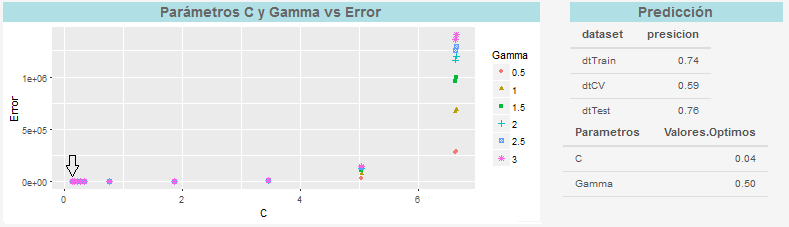
\includegraphics[width=0.8\linewidth]{images/SVM-sigmoide-2-flecha} 

}

\caption{Results of SVM with sigmoide kernel}\label{fig:SVM-sigmoide-2-flecha}
\end{figure}

The Table \ref{tab:results-of-efficiency-svm} show a comparative
framework of results of the four kernels that were tested. We can
observe that the sigmoid and radial are the best evaluated with a slight
advantage of 3 percentage points of the sigmoid over the radial. The
linear kernel is not a bad choice if one thinks in terms of simplicity
to program it and the little memory and processor that consumes.

\begin{table}[ht]
\centering
\caption{Results of officiency in prediction with SVM algorithm}
\label{tab:results-of-efficiency-svm}
\begin{tabular}{lllll}
\hline
                         & Lineal degree one & Lineal degree two & Radial & Sigmoide \\ \hline
Training dataset         & 72 \%             & 69 \%             & 80 \%  & 74 \%    \\
Cross Validation dataset & 70 \%             & 78 \%             & 69 \%  & 59 \%    \\
Test dataset             & 71 \%             & 67 \%             & 73 \%  & 76 \%    \\
Parameter C              & 0.04              & 0.14              & 0.40   & 0.04     \\
Parameter Gamma          & 0.5               & 0.5               & 0.5    & 0.5      \\ \hline
\end{tabular}
\end{table}

The Table \ref{tab:results-of-efficiency-svm}, also presents the best C
and Gamma parameters that the cross validation process selected for
these algorithm with different kernels, the parameter Gamma maintains
its value in each one of the two kernels that is required (radial and
sigmoide), 0.5 is the best value among the six values tested. On the
other hand, the parameter C, shows that small values are more
appropriate than big values. For C parameter, the best value is 0.40 for
Radial kernel and 0.04 for sigmoide kernel. C was chosen in a range of
0.01 to 1000. It means that in both cases the algorithm selected a wide
margin classifier.

\section{Comparing the results of the three algorithms and their
variants}\label{comparing-the-results-of-the-three-algorithms-and-their-variants}

All models that were trained with four factors exceed the precision of
the prediction to the models that were trained with the 21 factors
considered in the applied survey (see Table
\ref{tab:results-of-all-algoritms}). The mean of the prediction in the
models trained by the 21 factors is \(\mu=\) 63.33 with a standard
deviation of \(\sigma=\) 2.45, less than in the models trained with the
four factors selected by the algorithms described in Section
\ref{feature-selection} is \(\mu=\) 70.33 and standard deviation of
\(\sigma =\) 2.64.

\begin{table}[ht]
    \centering
    \caption{Results of all algorithms tested}
    \label{tab:results-of-all-algoritms}
    \begin{tabular}{llrrrrrr}
        \hline
        \multicolumn{1}{c}{\textbf{Algorithm}}  & \multicolumn{1}{c}{\textbf{Variant}} & \multicolumn{1}{p{1.5cm}}{\textbf{Features}} & \multicolumn{1}{c}{\textbf{Precision}} & \multicolumn{1}{p{1cm}}{\textbf{Time (sec)}} & \multicolumn{1}{p{1.5cm}}{\textbf{Features}} & \textbf{Precision} & \multicolumn{1}{p{1cm}}{\textbf{Time (sec)}} \\ \hline
        \multirow{2}{*}{ANN} & 3 Neurons    & 21  & 64\%  & 0.14   & 4  & 71\%   & 16.40   \\
                             & 4 Neurons    & 21  & 64\%  & 0.15   & 4  & 76\%   & 24.32    \\ \hline
        \multirow{3}{*}{LR}  & Linear, dg 1 & 21  & 66\%  & 0.25   & 4  & 71\%   & 0.59      \\
                             & Linear, dg 2 & 21  & 68\%  & 0.30   & 4  & 70\%   & 0.78       \\
                             & Linear, dg 3 & 21  & 60\%  & 0.70   & 4  & 64\%   & 4.44       \\ \hline
        \multirow{4}{*}{SVM} & Linear, dg 1 & 21  & 62\%  & 132.53 & 4  & 71\%   & 11.90      \\
                             & Linear, dg 2 & 21  & 62\%  & 147.21 & 4  & 69\%   & 12.46   \\
                             & Radial       & 21  & 62\%  & 20.47  & 4  & 73\%   & 8.11    \\
                             & Sigmoid      & 21  & 62\%  & 15.94  & 4  & 68\%   & 7.48   \\ \hline
    \end{tabular}
\end{table}

After obtaining these results, we decided to use only the four factors
selected to train the model for the estimation of sleep quality. The
next step is to choose the algorithm to be used for model generation.
The metrics that will be used to choose the algorithm will be, precision
of prediction, computational cost, implementation complexity in a mobile
device, and the flexibility of scaling in The time required. In the
table \ref{tab:results-of-all-algoritms}) we can see that the ANN of
four neurons and the SVM with radial kernel are the best algorithms in
prediction, however, the execution time are also of the highest. In
terms of implementation, the simplest is the LR and we can see that the
LR-trained model is below the SVM only two percentage points, and five
percentage points below the ANN Of four neurons in the hidden layer.
This allows us to have a preliminary idea of what should be done,
however it is necessary to do more tests to arrive at more solid
conclusions.

\chapter{Final Words}\label{final-words}

To be continued.

\bibliography{packages,book}


\end{document}
